%%%%%%%%%%%%%%%%%%%%%%%%%%%%%%%%%%%%%%%%%%%%%%%%%%%%%%%%%%%%%%%%%%%%%%%%%%%%%%%
% LAMMPS
%%%%%%%%%%%%%%%%%%%%%%%%%%%%%%%%%%%%%%%%%%%%%%%%%%%%%%%%%%%%%%%%%%%%%%%%%%%%%%%

\documentclass[aspectratio=169]{beamer}

\usepackage{fancyvrb}
\usepackage{graphicx}
\usepackage{hyperref}
\usepackage{listings}
\usepackage{xcolor}

%%%%%%%%%%%%%%%%%%%%%%%%%%%%%%%%%%%%%%%%%%%%%%%%%%%%%%%%%%%%%%%%%%%%%%%%%%%%%%%
% CONFIGURATION
%%%%%%%%%%%%%%%%%%%%%%%%%%%%%%%%%%%%%%%%%%%%%%%%%%%%%%%%%%%%%%%%%%%%%%%%%%%%%%%

\hypersetup{%
	colorlinks      = true,
	linkbordercolor = {white},
	urlcolor        = {blue}
}

\colorlet{codebg}{lightgray!30}

\AtBeginSection[]{
  \begin{frame}
  \vfill
  \centering
  \begin{beamercolorbox}[sep=8pt,center,shadow=true,rounded=true]{title}
    \usebeamerfont{title}\insertsectionhead\par%
  \end{beamercolorbox}
  \vfill
  \end{frame}
}

%%%%%%%%%%%%%%%%%%%%%%%%%%%%%%%%%%%%%%%%%%%%%%%%%%%%%%%%%%%%%%%%%%%%%%%%%%%%%%%
% LISTINGS LAMMPS
%%%%%%%%%%%%%%%%%%%%%%%%%%%%%%%%%%%%%%%%%%%%%%%%%%%%%%%%%%%%%%%%%%%%%%%%%%%%%%%

\lstdefinelanguage{LAMMPS}{%
	alsodigit       = {-},
	basicstyle      = \ttfamily,
	backgroundcolor = \color{codebg},
    keywordstyle    = [1]\color{magenta},
    keywordstyle    = [2]\color{blue},
    keywordstyle    = [3]\color{violet},
    keywordstyle    = [4]\color{orange},
    numberstyle     = \color{magenta},
    stringstyle     = \color{olive}\ttfamily,
    morestring      = [b]',
    morestring      = [b]",
	morecomment     = [f][\color{red}][0]{\#},
    keywords        = [1]{
        addforce,
        deposit,
        enforce2d,
        image,
        langevin,
        nve,
        recenter,
        setforce,
        shake,
        temp
    },
	keywords        = [2]{%
		atom_style,
		boundary,
        compute,
		create_atoms,
		create_box,
        delete_atoms,
		dimension,
		dump,
        fix,
        fix_modify,
        group,
		include,
        lattice,
		mass,
        minimize,
        molecule,
		neigh_modify,
		pair_coeff,
		pair_style,
        read_data,
		region,
        run,
        set,
        thermo,
        thermo_modify,
        timestep,
		units,
        variable,
        velocity,
        write_data
	},
    keywords        = [3]{%
        count
    },
    keywords        = [4]{%
        all,
        equal
    },
    otherkeywords  = {
        &,
        ave/time,
        lj/cut,
        lj/cut/tip4p/long,
        pppm/tip4p,
        temp/berendsen
    }
}

%%%%%%%%%%%%%%%%%%%%%%%%%%%%%%%%%%%%%%%%%%%%%%%%%%%%%%%%%%%%%%%%%%%%%%%%%%%%%%%
% COMMANDS
%%%%%%%%%%%%%%%%%%%%%%%%%%%%%%%%%%%%%%%%%%%%%%%%%%%%%%%%%%%%%%%%%%%%%%%%%%%%%%%

\newcommand\LAMMPS{%
	\href{https://www.lammps.org/}{LAMMPS}}

\newcommand\lammpsInline[1]{%
	\lstinline[language=LAMMPS]|#1|}

\newcommand\lammpsDocs[1]{%
	\lammpsInline{#1} (\href{https://docs.lammps.org/#1.html}{docs})}

%%%%%%%%%%%%%%%%%%%%%%%%%%%%%%%%%%%%%%%%%%%%%%%%%%%%%%%%%%%%%%%%%%%%%%%%%%%%%%%
% TITLE PAGE
%%%%%%%%%%%%%%%%%%%%%%%%%%%%%%%%%%%%%%%%%%%%%%%%%%%%%%%%%%%%%%%%%%%%%%%%%%%%%%%

\title{LAMMPS}
\subtitle{Molecular Dynamics simulator}
\author{Walter Dal'Maz Silva}
\date{\today}

%%%%%%%%%%%%%%%%%%%%%%%%%%%%%%%%%%%%%%%%%%%%%%%%%%%%%%%%%%%%%%%%%%%%%%%%%%%%%%%
% DOCUMENT
%%%%%%%%%%%%%%%%%%%%%%%%%%%%%%%%%%%%%%%%%%%%%%%%%%%%%%%%%%%%%%%%%%%%%%%%%%%%%%%

\begin{document}
\maketitle

\section{LAMMPS Introduction}
\begin{frame}{\secname}
This document describes the usage of \LAMMPS\ from beginner to advanced levels. No prior knowledge of the software is assumed. We will not strictly follow any references as the tutorials you find in this repository, but sometimes the order of some topics might seem related to those. For the external references, please consult the tutorial folders with proper links to their original sources.

\vspace{1cm}

Recommended operating system for learning \LAMMPS\ is Ubuntu under which you can install the software by running (with root rights) \Verb|sudo apt install lammps|. Test if it worked with \Verb|lmp -help|.

\vspace{1cm}

Installation under Windows is simple for single core and might get tricky if you wish to profit from parallelism. You can find more information \href{https://packages.lammps.org/windows.html}{here}.
\end{frame}

\begin{frame}{\secname}{Script structure}
The overall structure of a typical \LAMMPS\ script is the following:

\vspace{0.5cm}

\begin{description}
\item[Initialization]\hfill\\
Provides things as unit system, dimensionality, atomic style, bond style, interaction models, boundary conditions, ...
%
\item[System definition]\hfill\\
Declares regions, lattices, create atoms, place atoms in regions, load initialized data, ...
%
\item[Simulation settings]\hfill\\
Provides mass to atoms, describes pair interactions, deals on how to manage list of neighbors, apply fixes, ...
%
\item[Simulation run]\hfill\\
Set verbosity levels, declare data file dumps, provide integration parameters such as time step, ...
\end{description}
\end{frame}

\begin{frame}[fragile]{\secname}{Script structure}
Often \LAMMPS\ tutorials will teach you at a later point about \emph{snippet inclusion} in \LAMMPS\ scripts. It happens that if you learn about it earlier you can prevent many possible mistakes when dealing with multi-step calculations. Assume you have a subdirectory \Verb|config/| inside your computation project. You can place small text files with parts that are shared between several scripts using the keyword \lammpsInline{include} (\href{https://docs.lammps.org/include.html}{docs}):

\vspace{1cm}

\begin{lstlisting}[language={LAMMPS}]
# This is a comment in LAMMPS syntax.
# Next line includes some external script.
include    config/initialization.lammps
\end{lstlisting}

\vspace{1cm}

From now on we will make use of this feature whenever useful.
\end{frame}

\begin{frame}{\secname}{Script structure}
In many cases the order of command calls in \LAMMPS\ matters and one shall pay close attention to these situations. Examples include the declaration of geometric regions selecting part of space without previous definition of a box or the fact that some commands will provide additional configuration for the last declared lattice. This will become evident in the context and whenever possible you will be warned about.
\end{frame}

\begin{frame}[fragile]{\secname}{Running simulations}
The most simple way of running sequential \LAMMPS\ from command line is

\begin{verbatim}
> lmp -in <script_file_path>
\end{verbatim}

\noindent{}where \Verb|>| represents a command prompt and \Verb|<script_file_path>| is generally a file with the \Verb|.lammps| extension. If parallelism is available (and for any serious MD simulation you will need it) you can specify the number of processors with

\begin{verbatim}
> mpiexec -np <number_of_cores> lmp -in <script_file_path>
\end{verbatim}

Other command line options will be explored when required.
\end{frame}

\endinput


\section{Lennard-Jones Fluid}
\begin{frame}{\secname}
To start with our learning path, let's take the dimensionless Lennard-Jones fluid as an example. We will make a rephrasing of \href{https://lammpstutorials.github.io/tutorials/01-SimpleMolecularSimulation.html}{this tutorial}. Our refactored code can be found \href{https://github.com/WallyTutor/learning-scientific-computing/tree/main/molecular-dynamics/lammps/tutorials-simon-gravelle/01-Lennard-Jones-Mixture}{here} and you are invited to check its contents in case of doubts.

\vspace{0.5cm}

The study will be comprised of three major steps:

\vspace{0.5cm}

\begin{enumerate}
\item System creation and energy minimization for achieving a consistent initial state.
\item Integration of motion with a proper velocity distribution and some other fixes.
\item Modification of the case to apply global flow to the system.
\end{enumerate}

\vspace{0.5cm}

All steps will make use of the same initialization and thus we make use of the \lammpsInline{include} mechanism to keep it all in a single place.
\end{frame}

\begin{frame}[fragile]{\secname}{\subsecname}
In what follows we will model a 2D box with fixed size and filled with 1000 particles of type {I} and 500 particles of type {II}. The latter occupy initially a restricted cylinder in the center of the domain. Below we illustrate the random initialization, next the distribution after energy minimization, and finally the state by the end of simulation.

\vspace{0.5cm}

{%
\hfill%
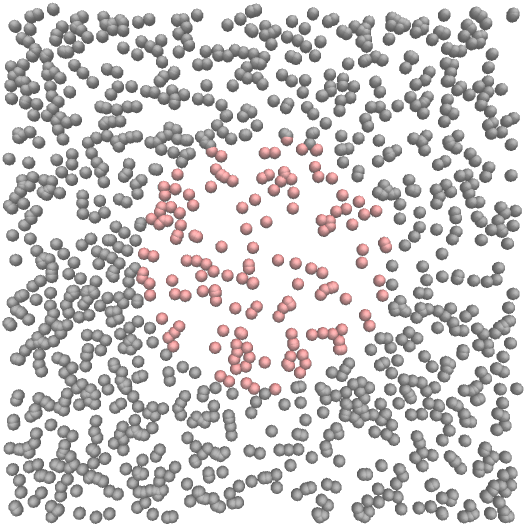
\includegraphics[width=3cm]{media/000-lennard-jones-init-random.png}
\hfill%
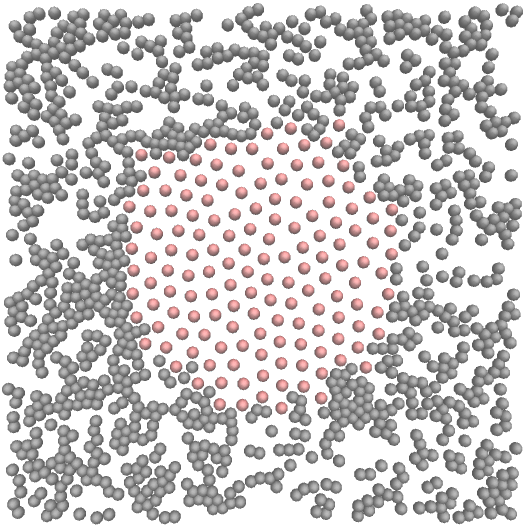
\includegraphics[width=3cm]{media/001-lennard-jones-init-minimized.png}
\hfill%
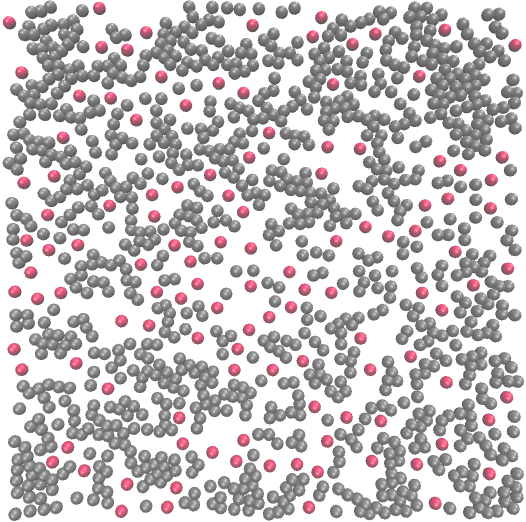
\includegraphics[width=3cm]{media/002-lennard-jones-final-state.png}
\hfill%
}
\end{frame}

\subsection{Initialization}

\begin{frame}[fragile]{\secname}{\subsecname\ - Unit system definition}
First of all, we define the \lammpsDocs{units} to be used in a simulation.

\vspace{0.5cm}

Different physical fields generally handle data with their units of choice so this has to be chosen compatible with the problem at hand. The default value \lammpsInline{lj} is strictly dimensionless.

\vspace{0.5cm}

\begin{lstlisting}[language=LAMMPS,basicstyle=\small]
# Specify unit system to use.
units        lj
\end{lstlisting}
\end{frame}

\begin{frame}[fragile]{\secname}{\subsecname\ - Simulation dimensions}
In \LAMMPS\, the simulation \lammpsDocs{dimension} is by default the 3D space.

\vspace{0.5cm}

It must be noted that just declaring a simulation to be 2D here is not enough and \href{https://docs.lammps.org/Howto_2d.html}{additional steps} are required to enforce physical constraints.

\vspace{0.5cm}

\begin{lstlisting}[language=LAMMPS,basicstyle=\small]
# Set the dimensionality of the simulation.
dimension    2
\end{lstlisting}
\end{frame}

\begin{frame}[fragile]{\secname}{\subsecname\ - Atomic style}
Command \lammpsDocs{atom_style} determines what attributes are associated with the atoms (and thus how the system definition is carried out later).

\vspace{0.5cm}

One must use the most generic style required to represent all particles in simulation since a more complex type also has the attributes of simpler ones.

\vspace{0.5cm}

\begin{lstlisting}[language=LAMMPS,basicstyle=\small]
# Determines attributes are associated with the atoms.
atom_style   atomic
\end{lstlisting}

\vspace{0.5cm}
In the present case most basic constituent \lammpsInline{atomic} is selected.
\end{frame}

\begin{frame}[fragile]{\secname}{\subsecname\ - Pair style}
Command \lammpsDocs{pair_style} provides what model is to be used to compute pairwise (in some cases even multi-body, please refer to the docs) interaction potential.

\vspace{0.5cm}

Given the large number of available models, \LAMMPS\ documentation provides a \href{https://docs.lammps.org/pairs.html}{dedicated section}. Notice that many of these models are domain-specific and only experience and external references can guide you on how to select the good one.

\vspace{0.5cm}

\begin{lstlisting}[language=LAMMPS,basicstyle=\small]
# Set how pairwise interactions are computed.
pair_style   lj/cut 2.5
\end{lstlisting}

\vspace{0.5cm}
Here a Lennard-Jones interaction with a cut-off potential of 2.5 is applied.
\end{frame}

\begin{frame}[fragile]{\secname}{\subsecname\ - Boundary}
Using \lammpsDocs{boundary} one specifies how the system interacts with its boundaries.

\vspace{0.5cm}

When simulating the behavior of a small fluid volume, it is reasonable in general to assume all boundaries are periodic, what approximates an infinite fluid domain.

\vspace{0.5cm}

\begin{lstlisting}[language=LAMMPS,basicstyle=\small]
# Set the type of boundary conditions on box sides.
boundary     p p p
\end{lstlisting}

\vspace{0.5cm}
In this case we apply all periodic boundary conditions.
\end{frame}

\begin{frame}[fragile]{\secname}{\subsecname\ - Include file}
With the elements of the previous slides we prepare the following include snippet that will be shared across the project steps.

\vspace{0.5cm}

\begin{lstlisting}[language=LAMMPS,basicstyle=\tiny]
# Specify unit system to use.
units        lj

# Set the dimensionality of the simulation.
dimension    2

# Determines what attributes are associated with the atoms.
atom_style   atomic

# Set how pairwise interactions are computed.
pair_style   lj/cut 2.5

# Set the type of boundary conditions on box sides.
boundary     p p p
\end{lstlisting}
\end{frame}

\subsection{System definition}

\begin{frame}[fragile]{\secname}{\subsecname\ - Declare region}
Quite often the first step in the system definition is the declaration of a bounded \lammpsDocs{region} of the space.

\vspace{0.5cm}

The syntax of this command depends on the \emph{style} provided by the second argument. Here with a block the values represent the bounds over $x$, $y$, and $z$ coordinate axes in Cartesian space.

\vspace{0.5cm}

\begin{lstlisting}[language=LAMMPS,basicstyle=\small]
# Defines a `block` region of space called `domain`.
region       domain block -30 30 -30 30 -0.5 0.5
\end{lstlisting}
\end{frame}

\begin{frame}[fragile]{\secname}{\subsecname\ - Create box}
Once space is delimited, one creates a simulation box with \lammpsDocs{create_box}.

\vspace{0.5cm}

In the present case we state that there will be 2 types of atoms in the region called \Verb|domain| previously defined.

\vspace{0.5cm}

\begin{lstlisting}[language=LAMMPS,basicstyle=\small]
# Simulation box with 2 atoms in region `domain`.
create_box   2 domain
\end{lstlisting}
\end{frame}

\begin{frame}[fragile]{\secname}{\subsecname\ - Create atoms}
We can then place atoms in the system by using \lammpsDocs{create_atoms}.

\vspace{0.5cm}

The first argument is the type number, followed by the \Verb|random| style and its arguments, here the number of atoms, a generator seed and the name of a region where to place the atoms (defined in the included file).
\vspace{0.5cm}

\begin{lstlisting}[language=LAMMPS,basicstyle=\small]
# Create space regions for placing atoms inside `domain`.
include      "config/02-named-regions.lammps"

# Creates 1500 atoms of type `1`.
create_atoms 1  random  1500  341341  cylout

# Creates 100 atoms of type `2`
create_atoms 2  random   100  127569  cylin
\end{lstlisting}
\end{frame}

\begin{frame}[fragile]{\secname}{\subsecname\ - Selected regions}
In the previous step we saw the use of additional regions defined in an external shared file. Here we make use of the \Verb|cylinder| style to delimit parts of the simulation box.

\vspace{0.5cm}

This is one of the cases where the order of commands matter. You cannot create these regions without previously calling the \lammpsDocs{create_box} command.

\vspace{0.5cm}

\begin{lstlisting}[language=LAMMPS,basicstyle=\small]
# Create additional regions representing a cylinder
# inner and outer zones for atom manipulations.
region       cylin  cylinder z 0 0 15 INF INF side in
region       cylout cylinder z 0 0 15 INF INF side out
\end{lstlisting}
\end{frame}

\begin{frame}[fragile]{\secname}{\subsecname\ - Final block}
The previous settings being compiled and with help of included file \Verb|config/02-named-regions.lammps| we complete the system definition.

\vspace{0.5cm}
Listing below provides the full block of system definition.
\vspace{0.5cm}

\begin{lstlisting}[language=LAMMPS,basicstyle=\tiny]
# Defines a geometric `block` region of space called `domain`.
region       domain block -30 30 -30 30 -0.5 0.5

# Simulation box with 2 atoms in region `domain`.
create_box   2 domain

# Create space regions for placing atoms inside `domain`.
include      "config/02-named-regions.lammps"

# Creates 1500 atoms of type `1`.
create_atoms 1  random  1500  341341  cylout

# Creates 100 atoms of type `2`
create_atoms 2  random   100  127569  cylin
\end{lstlisting}
\end{frame}

\subsection{Simulation settings}

\begin{frame}[fragile]{\secname}{\subsecname\ - Atoms masses}
For the simple \Verb|atomic| \lammpsDocs{atom_style} only the \lammpsDocs{mass} of atoms needs to be defined. Notice first argument given atom type is the one used with \lammpsDocs{create_atoms} and this will be true in many other occasions we might see.

\vspace{0.5cm}

This command also supports wildcards such as \lammpsInline{mass * 1.0} or \lammpsInline{mass 3* 2.0} for setting masses of whole families of atoms.

\vspace{0.5cm}

\begin{lstlisting}[language=LAMMPS,basicstyle=\small]
# Set the mass for all atoms of one or more atom types.
mass         1  1.0
mass         2  1.0
\end{lstlisting}
\end{frame}

\begin{frame}[fragile]{\secname}{\subsecname\ - Pair coefficients}
Particle interaction potentials is provided by \lammpsDocs{pair_coeff} declarations. At least interactions of atoms of same kind must be provided (types provided by first two arguments). Interactions between different kinds of atoms are computed from geometric mean of Lennard-Jones parameters well depth and cross-section.

\vspace{0.5cm}

Other types of dissimilar atoms computations may be specified or specific interactions may be declared but will not be done in this introductory case.

\vspace{0.5cm}

\begin{lstlisting}[language=LAMMPS,basicstyle=\small]
# Specify the pairwise force field coefficients.
pair_coeff   1  1  1.0  1.0
pair_coeff   2  2  0.5  3.0
\end{lstlisting}
\end{frame}

\begin{frame}[fragile]{\secname}{\subsecname\ - Neighbor list update}
Sometimes the default management of neighbor list update is not enough to ensure all possible configurations remain physical. Using \lammpsDocs{neigh_modify} we can manage this to avoid what \LAMMPS\ will call \Verb|dangerous builds|, \emph{i.e.} atomic placements with overlapping or similar nonphysical scenarios.

\vspace{0.5cm}

\begin{lstlisting}[language=LAMMPS,basicstyle=\small]
# Rebuild the neighbor lists more often.
neigh_modify every 1 delay 5 check yes
\end{lstlisting}
\end{frame}

\begin{frame}[fragile]{\secname}{\subsecname\ - Final block}
The previous settings being compiled in file \Verb|config/03-settings-common.lammps| we add only a \lammpsDocs{dump} statement to configure steps to be written to file once the simulation is run.

\vspace{0.5cm}
Listing below provides the full block of simulation settings. Notice the use of an ampersand \& for splitting the \lammpsDocs{dump} statement across multiple lines.
\vspace{0.5cm}

\begin{lstlisting}[language=LAMMPS,basicstyle=\tiny]
# Describe atoms and interactions, etc.
include      "config/03-settings-common.lammps"

# Dump results to file for dynamics visualization.
dump         state_minimized all atom 10 &
             "dumps/step-1-dynamics.lammpstrj"
\end{lstlisting}
\end{frame}

\subsection{Run simulation}

\begin{frame}[fragile]{\secname}{\subsecname\ - Thermodynamics verbosity}
We reach the final step of simulation setup, the configuration to perform time integration. In this first script our aim is simply to minimize energy of initial state so that actual simulation can run without problems.

\vspace{0.5cm}

To follow the values of thermodynamic properties we make use of \lammpsDocs{thermo}.

\vspace{0.5cm}

\begin{lstlisting}[language=LAMMPS,basicstyle=\small]
# Print thermodynamic every 10 steps.
thermo       10
\end{lstlisting}
\end{frame}

\begin{frame}[fragile]{\secname}{\subsecname\ - Energy minimization}
Energy minimization is performed with command \lammpsDocs{minimize}. Process is repeated iteratively until at least one of the four command arguments convergence/stop criteria listed below is reached:

\vspace{0.5cm}

\begin{enumerate}
\item change in energy between two iterations is less than value.
\item maximum force between two atoms in the system is lower than value.
\item maximum number of iterations of minimizer.
\item maximum number of force/energy evaluations.
\end{enumerate}
\vspace{0.5cm}

\begin{lstlisting}[language=LAMMPS,basicstyle=\small]
# Minimize system energy for initialization.
minimize     1.0e-04  1.0e-06  1000  10000
\end{lstlisting}
\end{frame}

\begin{frame}[fragile]{\secname}{\subsecname\ - Write data}
After minimization we can call \lammpsDocs{write_data} to dump the state so that it can be used in several simulation variants.

\vspace{0.5cm}

This is particularly useful when minimization becomes costly and dumping the initial state only once for later reuse is useful. Otherwise we could have carried out the full simulation in this first step, and for this case it would be totally acceptable, but here we follow a non-orthodox learning path of doing things by thinking how they should be done in \emph{real world} the hard way.

\vspace{0.5cm}

\begin{lstlisting}[language=LAMMPS,basicstyle=\small]
# Dump final state of energy minimization step to file.
write_data   "dumps/step-1-restart.min.lammps"
\end{lstlisting}
\end{frame}

\subsection{System dynamics}

\begin{frame}[fragile]{\secname}{\subsecname\ - Restarting a simulation}
If you have followed the steps in previous slides and ran the simulation you have probably produced a minimized state for starting up other simulations. In \LAMMPS\ we always need to add the four basic steps described in the introduction to any particular script. That's why it is interesting to work from the beginning with included snippets.

\vspace{0.5cm}

Data from previous step is loaded here with \lammpsDocs{read_data} and the preceding \lammpsDocs{include} ensures same (compatible) initialization.

\vspace{0.5cm}

\begin{lstlisting}[language=LAMMPS,basicstyle=\small]
# Perform system initialization.
include      "config/01-initialize.lammps"

# Path to data file with initial energy minimization.
read_data    "dumps/step-1-restart.min.lammps"
\end{lstlisting}
\end{frame}

\begin{frame}[fragile]{\secname}{\subsecname\ - Cleaning up I}
During minimization steps some particles might have left the initial cylinder defined in \Verb|config/02-named-regions.lammps|. \LAMMPS\ provides mechanisms to create groups and delete atoms for fine manipulation.

\vspace{0.5cm}

We create a shared snipped \Verb|config/04-groups-common.lammps| for the clean up.

\vspace{0.5cm}

\begin{lstlisting}[language=LAMMPS,basicstyle=\small]
# Create space regions for placing atoms inside `domain`.
include      "config/02-named-regions.lammps"

# Create groups for filtering atoms from regions.
include      "config/04-groups-common.lammps"
\end{lstlisting}
\end{frame}

\begin{frame}[fragile]{\secname}{\subsecname\ - Cleaning up II}
The contents of \Verb|config/04-groups-common.lammps| are presented below. First we create groups of atoms and regions, then we intersect them to identify atoms that are outside the region they should be initialize, all with \lammpsDocs{group}. Finish by deleting them with \lammpsDocs{delete_atoms}.

\vspace{0.5cm}

\begin{lstlisting}[language=LAMMPS,basicstyle=\tiny]
# NOTE: check names of regions in `02-named-regions.lammps`.

# Create groups by atom types.
group        type1 type 1
group        type2 type 2

# Create groups by regions over domain.
group        incyl  region cylin
group        outcyl region cylout

# Create intesection groups (atoms 1 inside/atoms 2 outside).
group        type1in  intersect type1 incyl
group        type2out intersect type2 outcyl

# Delete atoms from intersection groups.
delete_atoms group type1in
delete_atoms group type2out
\end{lstlisting}
\end{frame}

\begin{frame}[fragile]{\secname}{\subsecname\ - Simulation settings}
To wrap-up the settings we include the shared snippet that you already know and add a dump of system states every 500 steps for later carrying out the post-processing.

\vspace{0.5cm}

\begin{lstlisting}[language=LAMMPS,basicstyle=\small]
# Describe atoms and interactions, etc.
include      "config/03-settings-common.lammps"

# Dump results to file for dynamics visualization.
dump         state_minimized all atom 500 &
             "dumps/step-2-dynamics.lammpstrj"
\end{lstlisting}
\end{frame}

\begin{frame}[fragile]{\secname}{\subsecname\ - Simulation settings}
Now we will start by introducing the concept of \lammpsDocs{variable} and \lammpsDocs{fix}. The first stores values for later evaluation in a symbol, compatible with many \LAMMPS\ commands. Fixes are operations performed to groups of atoms during time stepping or minimization. Let's delve into their details in next slides.

\vspace{0.5cm}

\begin{lstlisting}[language=LAMMPS,basicstyle=\small]
# Include some more settings for counting atoms.
include      "config/05-count-atoms.lammps"

# Save number of atoms over time every 1000 steps.
fix          at1 all ave/time 1000 1 1000 v_Nt1in v_Nt1ou &
                 file "dumps/step-2-no-type-1.dat"
fix          at2 all ave/time 1000 1 1000 v_Nt2in v_Nt2ou &
                 file "dumps/step-2-no-type-2.dat"
\end{lstlisting}
\end{frame}

\begin{frame}[fragile]{\secname}{\subsecname\ - Addendum variables}
File \Verb|config/05-count-atoms.lammps| contains the following code. To declare a \lammpsDocs{variable} one provides its name, a style (here \Verb|equal|) and the arguments. Operation \lammpsInline{count} is one of the many available for this command and allows for counting objects of a given identifier or group in a region.

\vspace{0.5cm}

\begin{lstlisting}[language=LAMMPS,basicstyle=\small]
# NOTE: check groups in `04-groups-common.lammps`
# and names of regions in `02-named-regions.lammps`.

# Create variables to count atoms in different regions.
variable     Nt1in equal count(type1,cylin)
variable     Nt1ou equal count(type1,cylout)
variable     Nt2in equal count(type2,cylin)
variable     Nt2ou equal count(type2,cylout)
\end{lstlisting}
\end{frame}


\begin{frame}[fragile]{\secname}{\subsecname\ - Addendum fixes}
A \lammpsDocs{fix} is also composed by an identifier, a group of atoms it applies to (here \lammpsInline{all}), and a style (here \lammpsInline{ave/time}) followed by its arguments. Styles for fixed have their own documentation, \emph{e.g} \href{https://docs.lammps.org/fix_ave_time.html}{\lammpsInline{ave/time}}, which will compute time averaged quantities.

\vspace{0.5cm}

In the following block we see that the variables introduced in previous slide are accessed by prepending their names with \Verb|v_|, as in \Verb|v_Nt1in|.

\vspace{0.5cm}

\begin{lstlisting}[language=LAMMPS,basicstyle=\small]
fix          at1 all ave/time 1000 1 1000 v_Nt1in v_Nt1ou &
                 file "dumps/step-2-no-type-1.dat"
\end{lstlisting}
\end{frame}

\begin{frame}[fragile]{\secname}{\subsecname\ - Run simulation}
Initialization, system definition, and settings provided, it is time to prepare the simulation to run. It is a good idea to ensure \lammpsDocs{velocity} distribution is compatible with temperature.

\vspace{0.5cm}

Below we enforce a Gaussian distributed velocity with no overall linear or angular momenta are applied to the system.
\vspace{0.5cm}

\begin{lstlisting}[language=LAMMPS,basicstyle=\small]
# Initial velocity distribution compatible with temperature.
velocity     all create 1.0 4928459 mom yes rot yes dist gaussian
\end{lstlisting}
\end{frame}

\begin{frame}[fragile]{\secname}{\subsecname\ - Run simulation}
Next we set the simulation to run with constant number of atoms, volume, and energy through \lammpsDocs{fix} \lammpsInline{nve}. During integration a \href{https://doi.org/10.1103/PhysRevB.17.1302}{Langevin thermostat} fix is applied to hold system temperature approximately constant.

\vspace{0.5cm}

Note that using constant NVE with Langevin algorithm will perform Brownian
dynamics (BD).

\vspace{0.5cm}

\begin{lstlisting}[language=LAMMPS,basicstyle=\small]
# Constant NVE time integration - Stoermer-Verlet time integration
fix          mynve all nve

# Langevin thermostat algorithm.
fix          mylgv all langevin 1.0 1.0 0.1 1530917 zero yes
\end{lstlisting}
\end{frame}

\begin{frame}[fragile]{\secname}{\subsecname\ - Run simulation}
We have already discussed that \href{https://docs.lammps.org/Howto_2d.html}{further measures} are required to ensure a simulation is performed in 2D. Here we provide the required \lammpsDocs{fix}.

\vspace{0.5cm}

\begin{lstlisting}[language=LAMMPS,basicstyle=\small]
# Ensure atoms do not move over z-axis (pure 2D simulation).
fix          myefn all enforce2d
\end{lstlisting}
\end{frame}

\begin{frame}[fragile]{\secname}{\subsecname\ - Run simulation}
We provide the \lammpsDocs{timestep}, verbosity control \lammpsDocs{thermo}, and ask the simulation to \lammpsDocs{run}`. You might be interested in dumping the final state for starting other simulations with \lammpsDocs{write_data}, as we did previously.

\vspace{0.5cm}

\begin{lstlisting}[language=LAMMPS,basicstyle=\small]
# Time step used during integration.
timestep     0.005

# Print thermodynamic every 1000 steps.
thermo       50000

# Number of time steps to run.
run          1500000

# Dump final state of simulation step to file.
write_data   "dumps/step-2-restart.min.lammps"
\end{lstlisting}
\end{frame}

\begin{frame}[fragile]{\secname}{\subsecname\ - Post-processing}
After running the script you can read generated files and generate some plots or other types of post-processing (see \href{http://www.ks.uiuc.edu/Research/vmd/}{VMD}). Below we illustrate the number of particles of each type inside the cylinder initialized with particles of type 2 only.

\vspace{0.5cm}

{%
\hfill
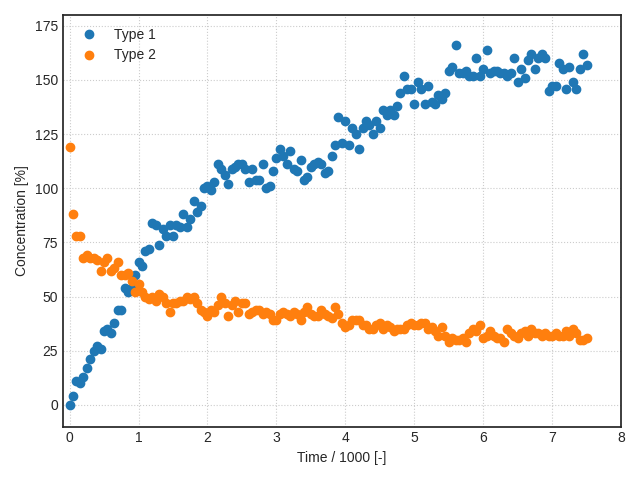
\includegraphics[width=7cm]{media/003-lennard-jones-concentration-evolution.png}
\hfill
}
\end{frame}

\begin{frame}[fragile]{\secname}{\subsecname\ - Next steps}
Some exercises are provided in the \href{https://lammpstutorials.github.io/tutorials/01-SimpleMolecularSimulation.html}{original source}.

\vspace{0.5cm}

What will happen if you add one more \lammpsDocs{fix} to add a net force with  \lammpsInline{addforce} to the system after the last fix we did previously?

\vspace{0.5cm}

\begin{lstlisting}[language=LAMMPS,basicstyle=\small]
# Experiment with imposed force to make particles flow.
fix          myfrc all addforce 1.0 0.0 0.0
\end{lstlisting}
\end{frame}

\endinput

\section{Permeable Membrane}
\begin{frame}[fragile]{\secname}
This tutorial deals with the osmosis through a semi-permeable membrane in 3D. So far you have already learned the basics of \LAMMPS\ and we will not provide all the code in this presentation, but only the blocks with new commands or explanations of how to do things differently. The full code can be found \href{https://github.com/WallyTutor/learning-scientific-computing/tree/main/molecular-dynamics/lammps/tutorials-simon-gravelle/02-Permeable-Membrane}{here}.

\vspace{0.5cm}

You may notice that we have not provided the \lammpsInline{units}, \lammpsInline{atom_style}, or \lammpsInline{dimension} in the scripts or snippets. That's because we will use default values adopted by \LAMMPS\, \lammpsInline{lj}, \lammpsInline{atomic}, \lammpsInline{3D}, respectively. We will also reduce the amount of comments around common commands.
\end{frame}

\begin{frame}[fragile]{\secname}
Getting proficient with \LAMMPS\ cases preparation requires careful thinking. In this tutorial, instead of taking you by the hand through the steps, we will reason about its structure. Some questions may arise, as follows:

\vspace{0.5cm}

\begin{itemize}
\item What's the system's geometry?
\item What atom and pair styles are suitable?
\item What other potentials should we use?
\item Which boundary conditions apply?
\item How many atom types do we need?
\item Are there forces/fixed parts?
\item What solution steps do we need?
\item ...
\end{itemize}
\end{frame}

\begin{frame}[fragile]{\secname}
So let's try to answer some of them and maybe ask ourselves a few more questions. Below we display the target system configuration.

\vspace{0.5cm}

There are 2 \emph{solid} walls enclosing the fluid, which is split into a left and right parts through a thin membrane. Solute atoms are added to the right side. If each wall has its atom type, plus one type for the solute and solved, we have a total of 5 atom types. Again we will consider a simple L-J interacting system.

\vspace{0.5cm}

{%
\hfill
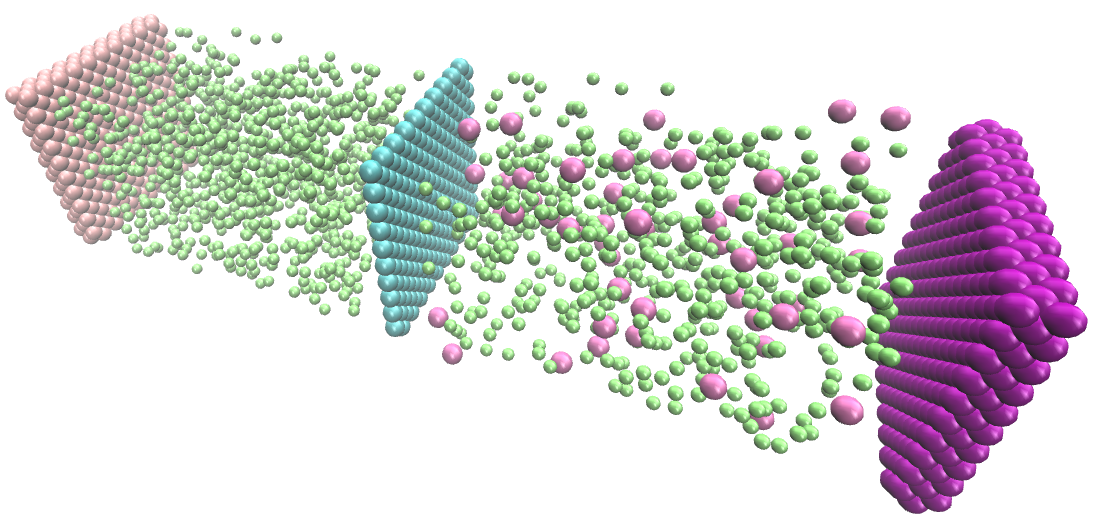
\includegraphics[width=7cm]{media/004-permeable-membrane-minimized.png}
\hfill
}
\end{frame}

\begin{frame}[fragile]{\secname}
Now we can stablish a solution strategy to tackle the problem:

\vspace{0.5cm}

\begin{enumerate}
\item First we create the system (walls, membrane, place atoms, set their properties) and call the minimization function to get a good starting point.

\item Next we run the simulation starting with minimized state. In this we fix membrane position and apply no forces to the walls, but leave them with a degree of freedom to move over $x$ axis, so that their position finds an equilibrium coordinate.

\item Finally, departing from the last state, we add some porosity to the membrane and simulate the osmotic pressure effect across the membrane.
\end{enumerate}

\vspace{0.5cm}

With that we already know that the project consists of 3 steps, the last 2 sharing most of the problem specification, thus using code snippets might be useful.
\end{frame}

\subsection{Initial minimization}

\begin{frame}[fragile]{\secname}{\subsecname\ - Initialization}
The system is initially not equilibrated. In fact we don't know where to specifically place the walls limiting the fluid.

\vspace{0.5cm}

In \LAMMPS\ this can be overcome with boundary condition type \lammpsInline{s}, which stands for \emph{shrink-wrapped}. With this condition the position of the box faces along are set so as to integrate the atoms in that dimension, no matter how far they move.

\vspace{0.5cm}

Below we apply it to the $x$ direction and also provide a \lammpsInline{lj/cut} cut-off potential.

\vspace{0.5cm}

\begin{lstlisting}[language=LAMMPS,basicstyle=\small]
boundary	 s p p
pair_style	 lj/cut 2.5
\end{lstlisting}
\end{frame}

\begin{frame}[fragile]{\secname}{\subsecname\ - Lattice creation}
To create the solid elements we need to specify a \lammpsDocs{lattice} prior to creating the region. There will be \lammpsInline{5} atom types in this simulation, one for each solid and two fluid species.

\vspace{0.5cm}

\begin{lstlisting}[language=LAMMPS,basicstyle=\small]
lattice       fcc 1
region        domain block  -23  23  -5  5  -5  5
create_box    5 domain
\end{lstlisting}
\end{frame}

\begin{frame}[fragile]{\secname}{\subsecname\ - Named regions}
As usual, its is practical to provided named regions.

\vspace{0.5cm}

Notice that they are unbounded in both $y$ and $z$ directions.

\vspace{0.5cm}

\begin{lstlisting}[language=LAMMPS,basicstyle=\tiny]
region        piston_left   block  -21.00  -20.00  INF  INF  INF  INF
region        fluid_left    block  -18.00   -2.00  INF  INF  INF  INF
region        membrane      block   -0.25    0.25  INF  INF  INF  INF
region        fluid_right   block    2.00   18.00  INF  INF  INF  INF
region        piston_right  block   20.00   21.00  INF  INF  INF  INF
\end{lstlisting}
\end{frame}

\begin{frame}[fragile]{\secname}{\subsecname\ - Filling the system}
If atoms are created in a region, they will occupy the lattice defined there.
Randomly placed atoms will form the fluid. It is this subtle difference that will define what atoms belong to each phase.

\vspace{0.5cm}

Notice that atom type \lammpsInline{4} (solvent) is used in both left and right fluids.

\vspace{0.5cm}

\begin{lstlisting}[language=LAMMPS,basicstyle=\tiny]
# Add atoms to what will be solid.
create_atoms  1 region piston_left
create_atoms  2 region membrane
create_atoms  3 region piston_right

# Add atoms to what will be fluid.
create_atoms  4 random 1000 654514  fluid_left
create_atoms  4 random 550  654514  fluid_right
create_atoms  5 random 50   424514  fluid_right
\end{lstlisting}
\end{frame}

\begin{frame}[fragile]{\secname}{\subsecname\ - Usage of wildcards}
If you have some experience with command line or scripting (and you should have some for managing your MD projects), you probably know what are \emph{wildcards}. \LAMMPS\ provides some support to them, but sometimes in unusual ways.

\vspace{0.5cm}

Below we set the mass of all atoms to unity by placing a star \lammpsInline{*} in place of atom indexes (what agrees with its usage in most \emph{nix} systems).

\vspace{0.5cm}

\begin{lstlisting}[language=LAMMPS,basicstyle=\small]
mass          * 1.0
\end{lstlisting}
\end{frame}

\begin{frame}[fragile]{\secname}{\subsecname\ - More on wildcards}
It is not always that \LAMMPS\ wildcard convention will match the typical. In the following snippet, the use of \lammpsInline{1*3  1*3} implies all pairwise combinations between atoms of types 1 to 3.

\vspace{0.5cm}

\begin{lstlisting}[language=LAMMPS,basicstyle=\small]
# Pair-wise coefficients.
pair_coeff    1*3  1*3  1.0  1.0
pair_coeff    4    4    1.0  1.0
pair_coeff    5    5    2.0  3.0
\end{lstlisting}

\vspace{0.5cm}

To confirm this, check section \Verb|PairIJ Coeffs| of restart file generated after running the first step of this tutorial.
\end{frame}

\begin{frame}[fragile]{\secname}{\subsecname\ - Overriding defaults}
We already discussed how \LAMMPS\ handles pair coefficients for interactions between atoms of different types. You can also enforce the values to take any user-defined values (and in more advanced cases, models).

\vspace{0.5cm}

Below we make interaction between solids and solvent \lammpsInline{4} / solute \lammpsInline{5} weaker, and also set the size of solute \lammpsInline{5} to a higher value to make membrane traversal less likely.

\vspace{0.5cm}

\begin{lstlisting}[language=LAMMPS,basicstyle=\small]
# Impose dissimetric coefficients for walls and solvent/solute.
pair_coeff    1*3  4    0.8  1.0
pair_coeff    1*3  5    0.1  3.0
\end{lstlisting}
\end{frame}

\begin{frame}[fragile]{\secname}{\subsecname\ - Run minimization}
This concludes the basic initialization and we can run the energy minimization followed by dump of restart file for what comes next.

\vspace{0.5cm}

\begin{lstlisting}[language=LAMMPS,basicstyle=\small]
thermo        10
minimize      1.0e-04  1.0e-06  1000  10000
write_data    "dumps/step-1-restart.min.lammps" pair ij
\end{lstlisting}
\end{frame}

\subsection{System equilibration}

\begin{frame}[fragile]{\secname}{\subsecname\ - Restarting from state}
By now you should be familiar with restarting a simulation from a dumped state. The following snipped illustrates how succinct it can be with use of included files, discussed in the next slides.

\vspace{0.5cm}

\begin{lstlisting}[language=LAMMPS,basicstyle=\tiny]
# Initialization -------------------------------------------------------------

include       "config/01-initialize.lammps"

# System definition ----------------------------------------------------------

read_data     "dumps/step-1-restart.min.lammps"
include       "config/02-system-definition.lammps"

# Simulation settings --------------------------------------------------------

include       "config/03-simulation-settings.lammps"
\end{lstlisting}
\end{frame}

\begin{frame}[fragile]{\secname}{\subsecname\ - Creating groups}
File \Verb|config/02-system-definition.lammps| is provided below. It simply provides groups for atom manipulations in upcoming steps.

\vspace{0.5cm}

The first \lammpsInline{neigh_modify} call is not necessary but will improve simulation performance by excluding the interactions between solid-solid atoms from updates of neighbor lists.

\vspace{0.5cm}

\begin{lstlisting}[language=LAMMPS,basicstyle=\tiny]
# Create region on right side of membrane for recording fluxes.
region       right block 0 INF INF INF INF INF

group        solid        type 1 2 3
group        fluid        type 4 5

group        piston_left  type 1
group        membrane     type 2
group        piston_right type 3
group        solvent      type 4
group        solute       type 5

neigh_modify exclude group solid solid
neigh_modify every 1 delay 5 check yes
\end{lstlisting}
\end{frame}

\begin{frame}[fragile]{\secname}{\subsecname\ - Simulation settings}
Simulation settings are shared by the initial equilibration being discussed here and the next step, the simulation run. You can check the contents of the included snippet file \href{https://github.com/WallyTutor/learning-scientific-computing/blob/main/molecular-dynamics/lammps/tutorials-simon-gravelle/02-Permeable-Membrane/config/03-simulation-settings.lammps}{\Verb|config/03-simulation-settings.lammps|} on the repository .

\vspace{0.5cm}

The only point I would like to discuss further here is the different between providing zero force or \lammpsInline{NULL}, the latter leaving a movement degree of freedom.

\vspace{0.5cm}

\begin{lstlisting}[language=LAMMPS,basicstyle=\tiny]
# Cancel forces on membrane to keep it fixed.
fix           mysf1 membrane setforce 0 0 0

# Freeze pistons but allow movement over x with NULL (leave a DoF).
fix           mysf2 piston_left  setforce NULL 0 0
fix           mysf3 piston_right setforce NULL 0 0
\end{lstlisting}
\end{frame}

\begin{frame}[fragile]{\secname}{\subsecname\ - Run equilibration}
To conclude this step, we add a few fixes to keep track of concentrations and piston positions. Simulation is run for a large number of steps aiming at initial equilibration.

\vspace{0.5cm}

\begin{lstlisting}[language=LAMMPS,basicstyle=\tiny]
fix           myat1 all ave/time 1000 1 1000 v_solvent_right         &
               file "dumps/step-2-solvent-right.dat"
fix           myat2 all ave/time 1000 1 1000 v_solute_right          &
               file "dumps/step-2-solute-right.dat"
fix           myat3 all ave/time 1000 1 1000 v_position_piston_left  &
               file "dumps/step-2-position-piston-left.dat"
fix           myat4 all ave/time 1000 1 1000 v_position_piston_right &
               file "dumps/step-2-position-piston-right.dat"

dump          mydmp all atom 1000 &
              "dumps/step-2-dynamics.lammpstrj"

thermo_modify temp temperature_fluid

# Run simulation -------------------------------------------------------------

thermo        10000
run           500000
write_data    "dumps/step-2-restart.min.lammps" pair ij
\end{lstlisting}
\end{frame}

\begin{frame}[fragile]{\secname}{\subsecname\ - Convergence check}
Before going further towards production run, we verify the pistons have found an equilibrium position, as illustrated below. This validates the initialization and we can advance to next steps.

\vspace{0.5cm}

{%
\hfill
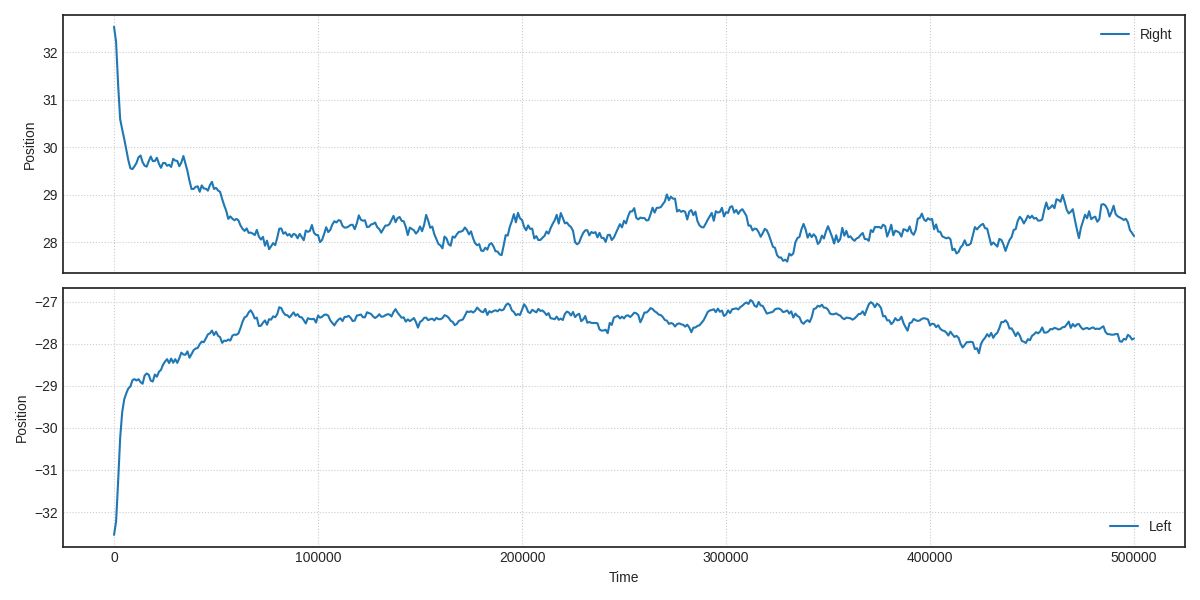
\includegraphics[width=8cm]{media/005-permeable-membrane-piston-position.png}
\hfill
}
\end{frame}

\subsection{Production run}

\begin{frame}[fragile]{\secname}{\subsecname\ - Making membrane porous}
Final script can be found \href{https://github.com/WallyTutor/learning-scientific-computing/blob/main/molecular-dynamics/lammps/tutorials-simon-gravelle/02-Permeable-Membrane/input-step-3.lammps}{here}. The only difference with regards to the system equilibration we just performed is the random deletion some atoms from the membrane, so that it is porous.

\vspace{0.5cm}

In newer versions of \LAMMPS\ you can delete the last 2 lines and comment out the second line of the following snippet.

\vspace{0.5cm}

\begin{lstlisting}[language=LAMMPS,basicstyle=\small]
# Delete 50% of atoms from membrane.
# delete_atoms random fraction 0.5 no all membrane 482793
region       membrane block -0.25 0.25 INF INF INF INF
delete_atoms porosity membrane 0.5 482793
\end{lstlisting}
\end{frame}

\begin{frame}[fragile]{\secname}{\subsecname\ - Final results}
If everything went well you probably got results similar to the following. With that we are ready to go to the next step!

\vspace{0.5cm}

{%
\hfill
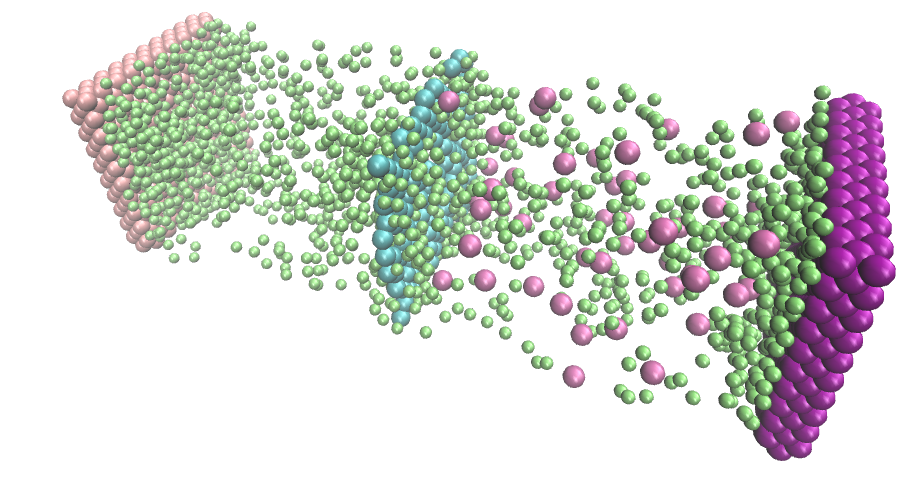
\includegraphics[width=6cm]{media/006-permeable-membrane-final.png}
\hfill
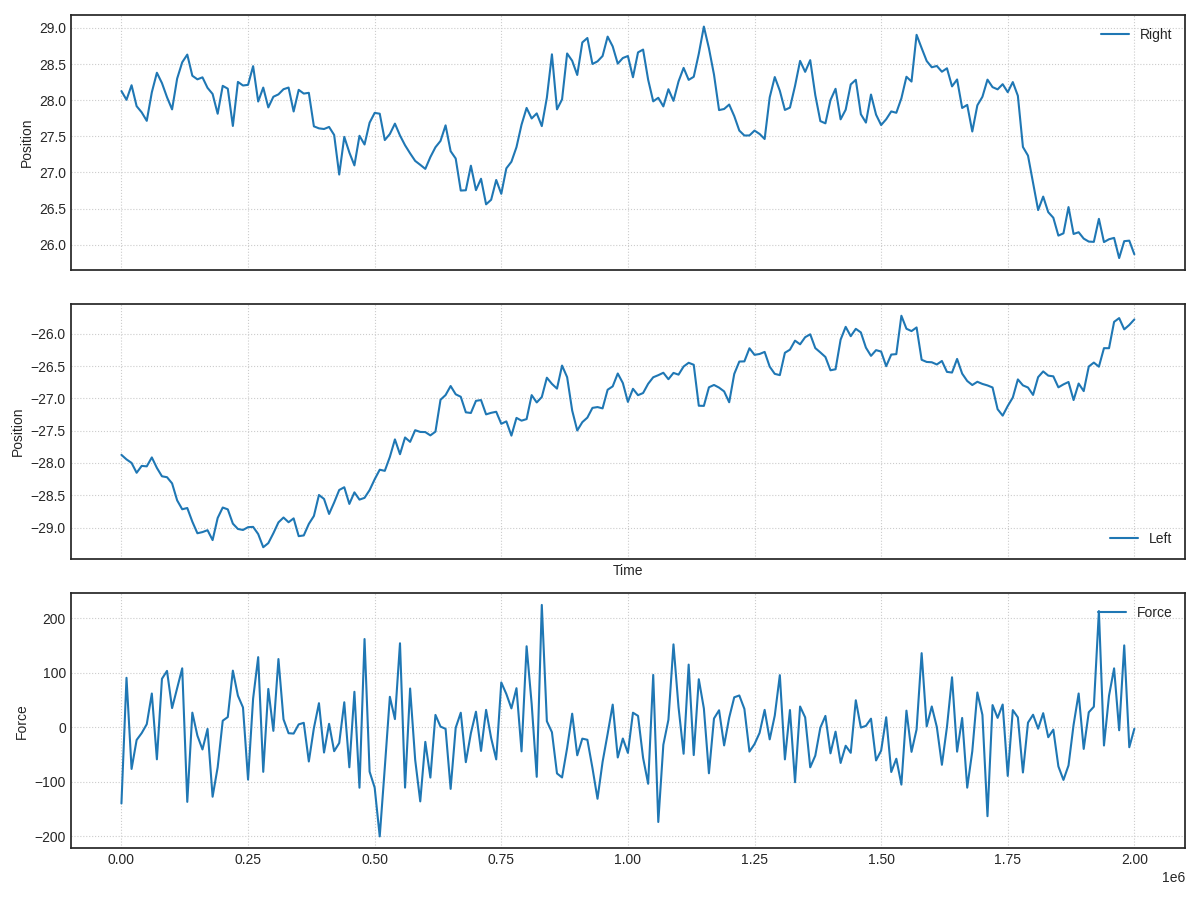
\includegraphics[width=6cm]{media/008-permeable-membrane-piston-position.png}
\hfill
}
\end{frame}

\endinput

\section{Nanoconfined Electrolyte}
\endinput

\section{Graphene Deformation}
\endinput

\section{Water Adsorption in Silica}
\endinput

\section{Free Energy Calculation}
\endinput

\end{document}